%

%%%%%%%%%%%%%%%%%%%%%%%%%%%%%%%%%%%%%%%%%%%%%%%%%%%%%%%%%%%%%%%%%%%%%%%%
\chapter{Plugin Implementation}
\label{chap:PluginImplementation}

\blindtext[1]

%%%%%%%%%%%%%%%%%%%%%%%%%%%%%%%%%%%%%%%%%%%%%%%%%%%%%%%%%%%%%%%%%%%%%%%%
\section{Goals}
\label{sec:goals}

\blindtext[2]

%%%%%%%%%%%%%%%%%%%%%%%%%%%%%%%%%%%%%%%%%%%%%%%%%%%%%%%%%%%%%%%%%%%%%%%%
\section{Implementation details}
\label{sec:implementationDetails}

\blindtext[1]

%%%%%%%%%%%%%%%%%%%%%%%%%%%%%%%%%%%%%%%%%%%%%%%%%%%%%%%%%%%%%%%%%%%%%%%%

\subsection{Key Features}
\label{sec:keyFeatures}

\blindtext[2]

\subsection{User Interface}
\label{sec:userInterface}

\blindtext[8]

\subsection{Architecture}
\label{sec:Architecture}

\blindtext[8]

%%%%%%%%%%%%%%%%%%%%%%%%%%%%%%%%%%%%%%%%%%%%%%%%%%%%%%%%%%%%%%%%%%%%%%%%

\section{Encountered Problems}
\label{sec:encounteredProblems}

In this section, I will discuss the main problems I encountered during implementation. To briefly summarize, they mainly consisted of how to create a simple, intuitive user interface and how the system behind the interface should be designed to have the best or at least a reasonable performance. \\ In the other visualizations, I noticed that I was quite overwhelmed by the amount of buttons which were visible, even though not always enabled. So I wanted to keep my user interface as simple as possible while not restricting the user in his ability to navigate through the visualization. \\ Regarding the performance, I have read in the thesis about the AES visualization that to create a fluent user experience where he can navigate back and forth between all steps, the intermediate values need to be calculated beforehand and saved since we don't want to stop at each step to calculate the next value or recalculate everything from the start if the user wants to go backwards.\\
I hope that the description of these problems and the solutions I have found may help future students in writing their own plugins.

\subsection{Performance}

The peformance of the plugin was essentially coupled to how the navigation system was designed. Other things like the calculation of the intermediate values for the visualization were unsignificant because they are created by the ChaCha cipher anyway and must just be saved somewhere to not lose them. I realized this relationship early in development when I had my first page with many page actions on it and wanted to skip ahead a lot of actions. While implementing this feature which would enable the user to skip from any action to any other action, I realized that when skipping more than 100 actions, it already took about 750ms during which the UI was unresponsive. As can be seen in FIGURE X, this time increased linearly so it was quite clear that I needed to do something about this, especially because the page with the most actions had over 3000 single actions.

\par

The root cause of the problem was the navigation system design which I called in hindsight \textbf{\textit{linear navigation system}}. It consisted of defining actions which build upon each other. This means that if we are at action 0 (initial state of the page) and want to go to action 5, we need to execute all the code inside the action definitions between 0 and 5 to arrive at the page state as it should be at action 5. This is resembled in Figure \ref{navsystem.linear.overview}.

\begin{figure}
\caption{Navigation paths between actions in the linear navigation system}
\label{navsystem.linear.overview}
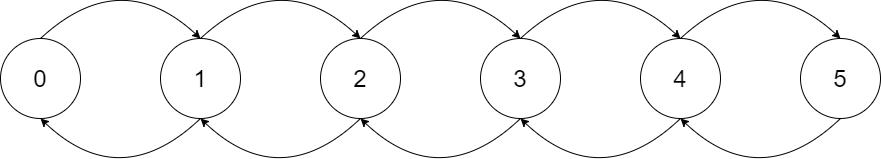
\includegraphics[width=\textwidth]{figures/navigationsystem-linear-overview.png}
\end{figure}

I came up with this design to have a smooth implementation experience where I only have to write the actual page state changes between two actions instead of duplicating a lot of code since the page state changes which were applied during a previous page were most of the times still visible when moving to the next action. This complements how the user experiences the visualization because the actions are numbered in a sequence and thus are inherently linear. Thus it made a lot of sense to me to reflect this in the system architecture.

\par

Since this "design flaw" was not the leading cause of the performance problem (going through a for-loop of size 3000 does not directly lead to performance issues), I want to briefly explain how the actual action implementation looked like.\\
As can be seen in Figure \ref{navsystem.linear.detail}, during the transition between two page states, the state of the page elements which will change is saved such that we can undo the changes if the user decides to navigate back. This enabled me to skip writing action definitions for backwards navigation, since I could just write a function which retrieves the state corresponding to the transition and then applies it. This function would then work for all backwards navigation without further intervention which was very convenient during development.

\par
